\documentclass[11pt]{article}
\usepackage[sc]{mathpazo} %Like Palatino with extensive math support
\usepackage{fullpage}
\usepackage[authoryear,sectionbib,sort]{natbib}
\linespread{1.7}
\usepackage[utf8]{inputenc}
\usepackage{lineno}
\usepackage{titlesec}
\titleformat{\section}[block]{\Large\bfseries\filcenter}{\thesection}{1em}{}
\titleformat{\subsection}[block]{\Large\itshape\filcenter}{\thesubsection}{1em}{}
\titleformat{\subsubsection}[block]{\large\itshape}{\thesubsubsection}{1em}{}
\titleformat{\paragraph}[runin]{\itshape}{\theparagraph}{1em}{}[. ]\renewcommand{\refname}{Literature Cited}

%ONES I ADDED
\usepackage{amsmath,amssymb} % For the math
\usepackage{url} % for easy url hyperlinks
%\bibliographystyle{amnatnat} % The bib style
\usepackage[]{graphicx,color,colortbl} % For the figs.

%%%%%%%%%%%%%%%%%%%%%
% Line numbering
%%%%%%%%%%%%%%%%%%%%%
%
% Please use line numbering with your initial submission and
% subsequent revisions. After acceptance, please turn line numbering
% off by adding percent signs to the lines %\usepackage{lineno} and
% to %\linenumbers{} and %\modulolinenumbers[3] below.
%
% To avoid line numbering being thrown off around math environments,
% the math environments have to be wrapped using
% \begin{linenomath*} and \end{linenomath*}
%
% (Thanks to Vlastimil Krivan for pointing this out to us!)

%%%%%%%%%%%%%%%%%%%%% THIS SHOULD REMOVED WHEN LINE NUMBERS ARE REMOVED %%%%%%%%%%%%%%%%%%%%%%%%%%%%%%%% THIS PIECE OF CODE IS WHAT SHOULD SOLVE THE ISSUE WITH LINE NUMBERS %%%%%%%%%%%%%%%%%%%%%%%%%%%

\newcommand*\patchAmsMathEnvironmentForLineno[1]{%
   \expandafter\let\csname old#1\expandafter\endcsname\csname #1\endcsname
   \expandafter\let\csname oldend#1\expandafter\endcsname\csname end#1\endcsname
   \renewenvironment{#1}%
      {\linenomath\csname old#1\endcsname}%
      {\csname oldend#1\endcsname\endlinenomath}}% 
\newcommand*\patchBothAmsMathEnvironmentsForLineno[1]{%
   \patchAmsMathEnvironmentForLineno{#1}%
   \patchAmsMathEnvironmentForLineno{#1*}}%
\AtBeginDocument{%
\patchBothAmsMathEnvironmentsForLineno{equation}%
\patchBothAmsMathEnvironmentsForLineno{align}%
\patchBothAmsMathEnvironmentsForLineno{flalign}%
\patchBothAmsMathEnvironmentsForLineno{alignat}%
\patchBothAmsMathEnvironmentsForLineno{gather}%
\patchBothAmsMathEnvironmentsForLineno{multline}%
}
%%%%%%%%%%%%%%%%%%%%%%%%%%%%%%%%%%%%%%%%%%%%%%%%%%%%%%%%%%%%%%%%%%%%%%%%%%%%%%%%%%%%%%%%%%%%%%%%%


\title{Rethinking the Road Effect Zone: The Probabilistic Effect of Roads on Ecosystems}

% This version of the LaTeX template was last updated on
% September 28, 2022.

%%%%%%%%%%%%%%%%%%%%%
% Authorship
%%%%%%%%%%%%%%%%%%%%%
% Please remove authorship information while your paper is under review,
% unless you wish to waive your anonymity under double-blind review. You
% will need to add this information back in to your final files after
% acceptance.

%\author{ Michael J. Noonan$^{1,\ast}$ \\
%Arnaud L. J. Desbiez$^{2,3,4}$ \\ 
%Adam T. Ford$^{1}$}

\date{}

\begin{document}

\maketitle

%\noindent{} 1. Department of Biology, The University of British Columbia, Okanagan Campus, British Columbia, Canada;
%
%\noindent{} 2. Instituto de Conservacão de Animais Silvestres (ICAS), Mato Grosso do Sul, Brazil;
%
%\noindent{} 3. Instituto de Pesquisas Ecológicas (IPÊ), São Paulo, Brazil.
%
%\noindent{} 4. Royal Zoological Society of Scotland (RZSS), Edinburgh, United Kingdom.
%
%\noindent{} $\ast$ Corresponding author; e-mail: michael.noonan@ubc.ca.

\bigskip

\textit{Manuscript elements}: Figure~1, figure~2, figure~3. Figure~1, 2, and 3 are to print in color.

\bigskip

\textit{Keywords}: Anthropocene, Anthropogenic impacts, GPS tracking, Home range, Movement ecology, Road ecology, Space use.

\bigskip

\textit{Manuscript type}: Note.

\bigskip

\noindent{\footnotesize Prepared using the suggested \LaTeX{} template for \textit{Am.\ Nat.}}

%\linenumbers{}
%\modulolinenumbers[3]

\newpage{}

\linenumbers

\section*{Abstract}

Roads are important for human socio-economic growth, but they carry substantial ecological impacts that can extend far beyond their physical footprint. These impacts have given rise to the so called `Road Effect Zone'. Although the foundational concept of the Road Effect Zone has proven useful in measuring patterns of biodiversity loss near roads, it focuses on changes in species presence/abundance, rather than the potential effects on ecological interactions. Here, we introduce a more mechanistic approach to the road effect zone that brings together the probability of a wildlife-vehicle collision with the probability of an ecological interaction occurring across an animal’s home range. We demonstrate the utility of a probabilistic representation of the road effect for giant anteaters living near a highway in Brazil. We then conclude with a brief discussion of how this probabilistic road effect can be employed in practice to inform species conservation.

\newpage{}


% ----------------------------------------------------------------
% Introduction
% ----------------------------------------------------------------

\section*{Introduction}

The ca. 64,000,000 km of roads distributed across the globe are important for human socio-economic growth \citep{Ibisch:2016}. Yet, while the area that roads occupy might be small, the ecological impacts they carry are substantial \citep{Coffin:2007, Fahrig:2009, Ascensao:2022}, and can extend far beyond their physical footprint \citep{Forman:1998, Forman:2003}. From an ecological perspective, roads and roadside ecotones are considered high disturbance systems with non-natural chemical, physical, hydrological, and auditory properties \citep{Reijnen:1996, Forman:1998, Brady:2017}. Roads have been shown to alter population densities \citep{Reijnen:1996, Fahrig:2009, Andrasi:2021}, community composition \citep{Truscott:2005}, evolutionary trajectories \citep{Brown:2013, Brady:2017}, and are a serious source of non-natural mortality for many species \citep{Desbiez:2020, Silva:2020, Carter:2020, Ascensao:2022}. Fully understanding the ecological footprint of roads is thus of the utmost importance if we are to design well-informed ecological mitigation strategies.

Roads can cause a broad range of ecological impacts, but their effects are usually considered strongest with increasing proximity to the road surface. The strength or impact of these road effects decay at varying rates with increasing distance from the road. This relationship between the strength of effect and proximity to the road forms the basis for the concept of the  `Road Effect Zone' \citep{Forman:1998, Forman:2000}, hereafter referred to as the REZ (Fig.~\ref{Fig:REZ}). Ecologists and conservation practitioners regularly quantify the REZ for different species \citep[e.g.,][]{Semlitsch:2007, Eigenbrod:2009, Andrasi:2021}, and these distances are often used to make conservation recommendations \citep[e.g.,][]{Forman:2000b, Peaden:2015, Ford:2020}.

\begin{figure}[h!]
\centering
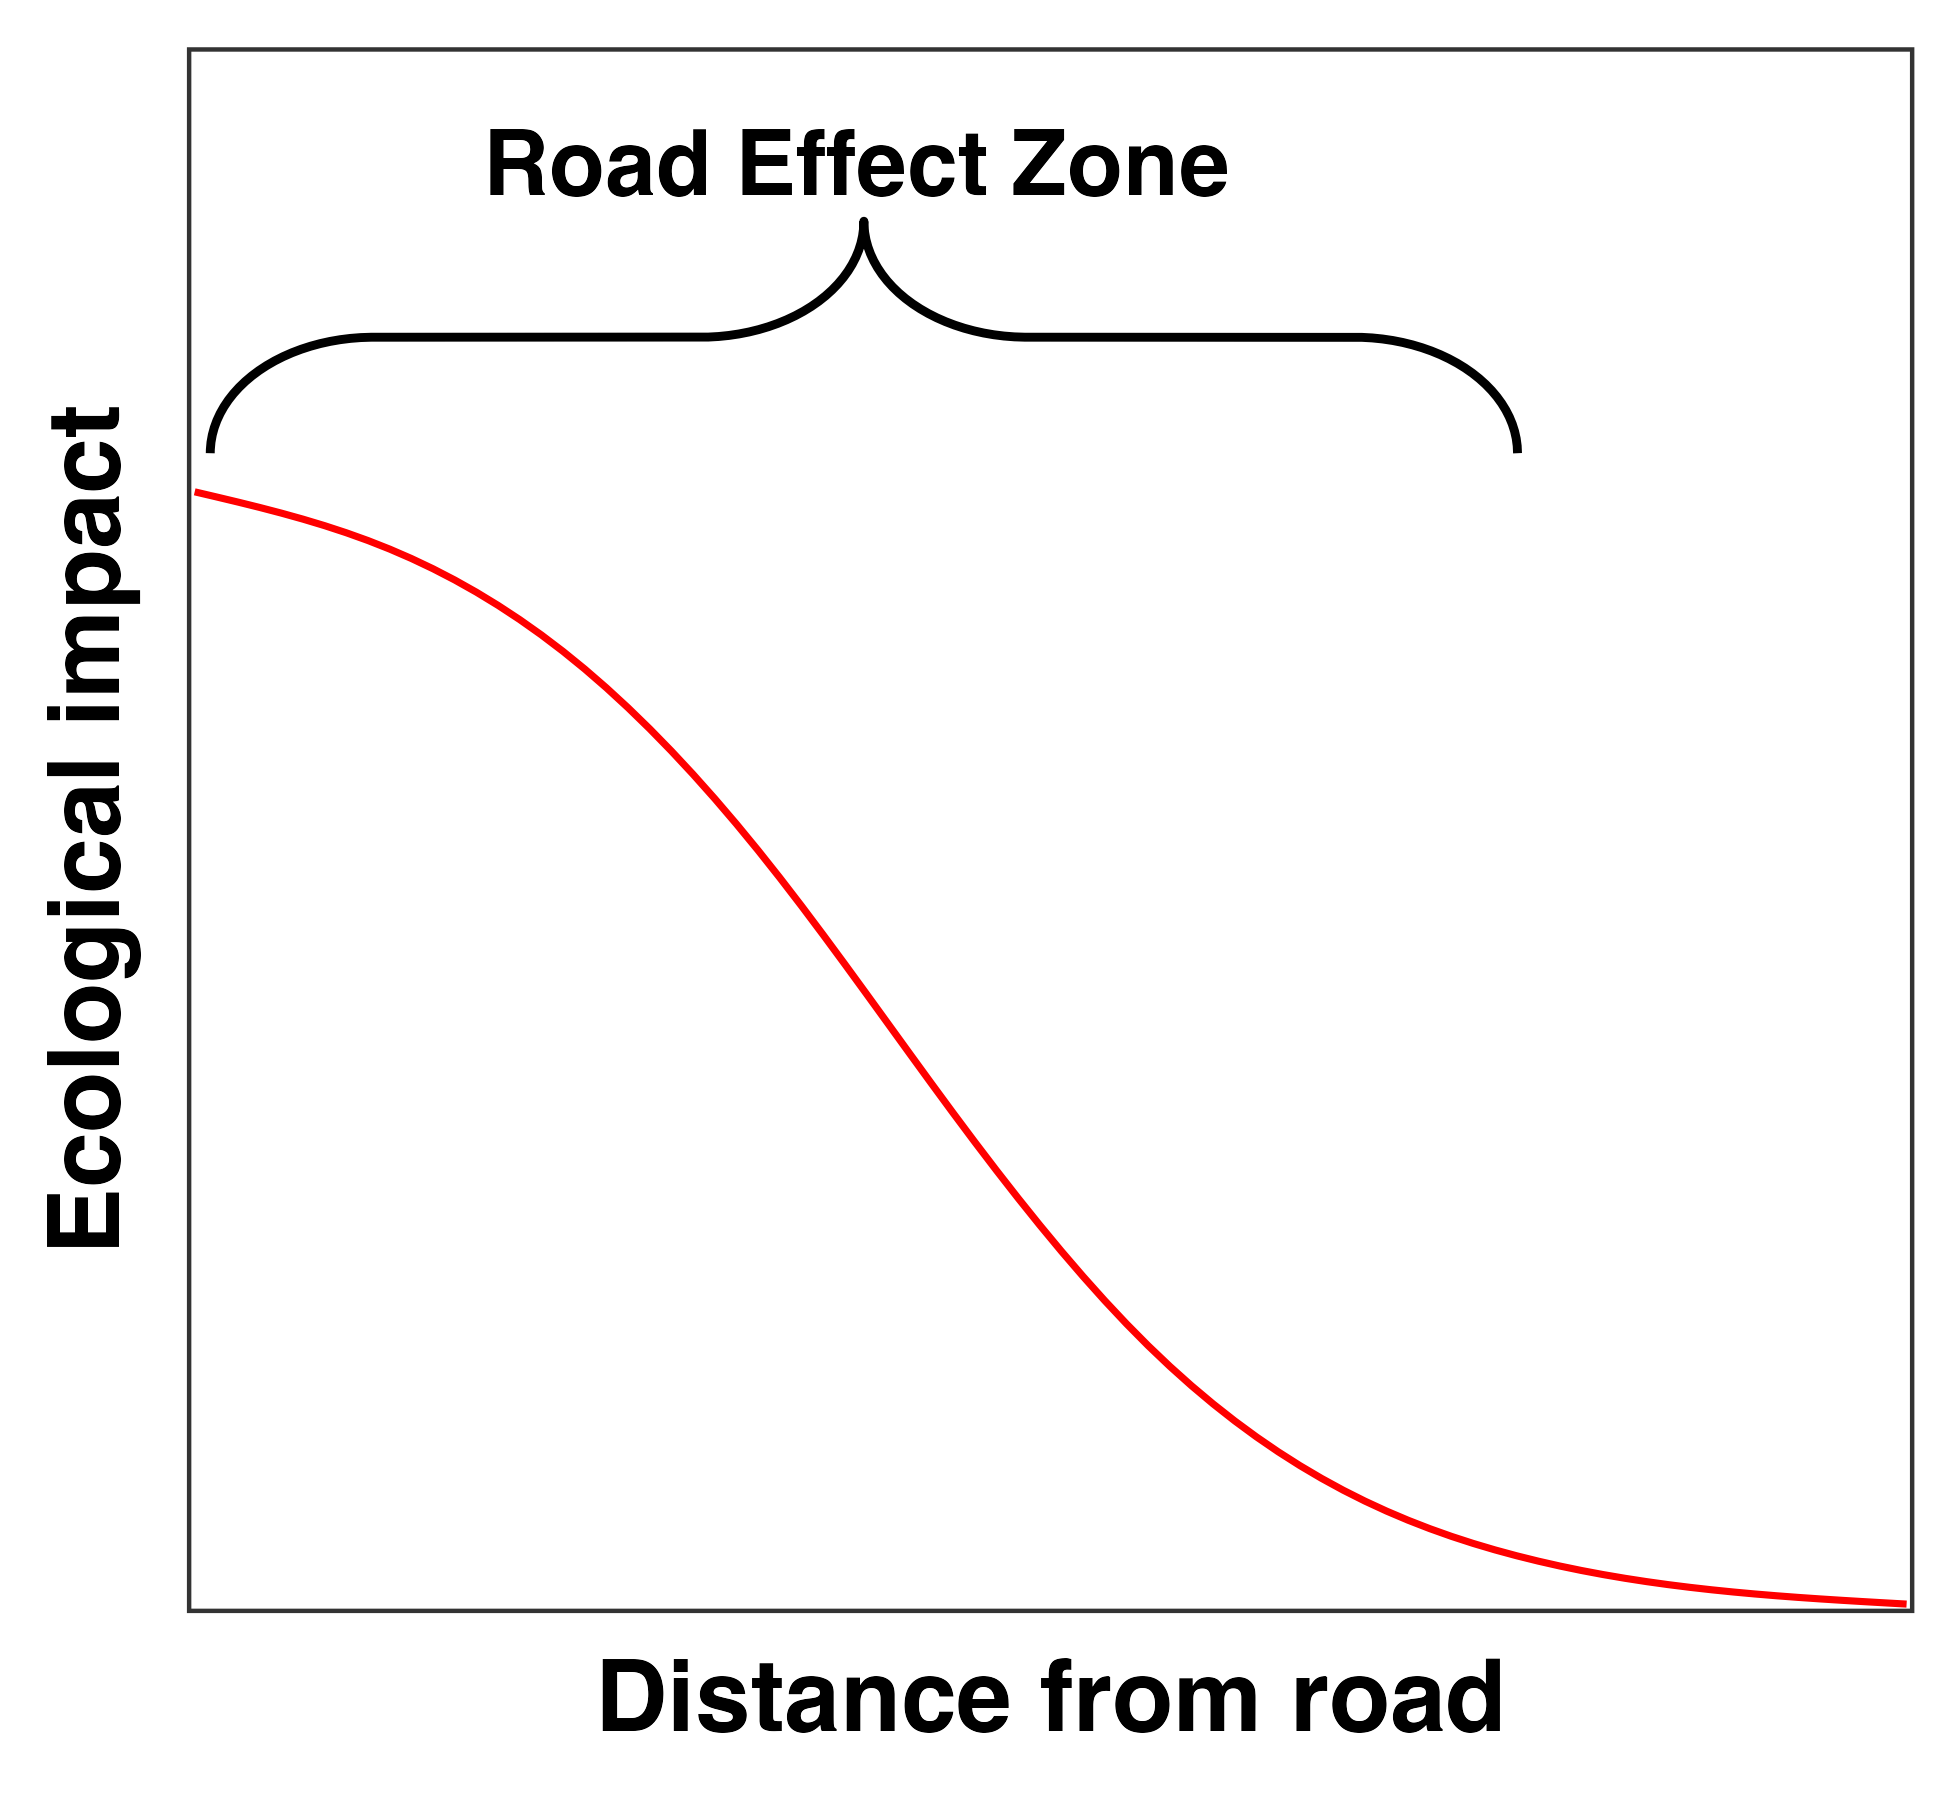
\includegraphics{REZ}
\caption{Theoretical depiction of the road effect zone as originally defined by \cite{Forman:1998}.}
\label{Fig:REZ}
\end{figure}

Although the REZ has proven useful in measuring patterns of biodiversity loss, it’s correlative basis combines several mechanisms that shape where and why roads affect nature. The REZ concept is also a static measure that does account for the dynamic effects animal movement and species interactions. This is a noteworthy limitation. Consider for instance, migratory ungulates that move over vast distance between seasonal home ranges \citep{Kauffman:2020, Kauffman:2021}. The effects of road mortality on these highly vagile animals might decrease nutrient transfer \citep{Subalusky:2017}, prey densities \citep{Walton:2017}, and/or grazing pressure \citep{Augustine:1998} hundreds or even thousands of kilometers away from the road, yet these effects would not be captured within the current REZ framework. Similarly, for territorial species, the death of a roadside animal can have a cascading effect on the species' socio-spatial arrangement over vastly larger distances than the conventional REZ might suggest as individuals disperse and restructure themselves around newly unoccupied territories \citep{Mumme:2000}. The reduction in density of frugivorous and/or seed-caching animals around roads can also have cascading effects on seed dispersal over larger areas than described by the REZ \citep{Tucker:2021}. Here, we introduce a more mechanistic probabilistic road effect (PRE) that describes the broader ecological impacts that the mortality of an animal might have on the landscape.


% ----------------------------------------------------------------
% The Road Effect as a Joint Probability
% ----------------------------------------------------------------

\section*{The Road Effect as a Joint Probability}

As noted above, our focus is on the ecological impact of a wildlife mortality caused by a collision with a vehicle. Our framework begins from the concept of animal space use and movement ecology. An individual's home range describes the space it uses to undergo `\textit{its normal activities of food gathering, mating, and caring for young}' \citep{Burt:1943he}. Ecologists have long recognised the utility of the home-range concept in describing patterns of space use \citep[e.g.,][]{Kie:2010es}, and routinely estimate home ranges from animal tracking data \citep[see][]{AKDEvsKDE}. Statistically, home-range estimation results in a probability distribution function ($\mathrm{PDF_{HR}}$) satisfying

\begin{equation}
\iint_{-\infty}^\infty \mathrm{PDF_{HR}}~dxdy = 1.
\end{equation}

The $\mathrm{PDF_{HR}}$ provides information on the locations where an animal is likely to be found. Importantly for the context of understanding the effects of roads on ecological processes, $\mathrm{PDF_{HR}}$ also represents the sample space over which an individual's ecological interactions (e.g., foraging, mating, defecating, engaging in territorial defence, etc.) are expected to occur. This PDF can thus be considered to be proportional to an animal's impact on or from the ecosystem, with core (i.e., high probability) areas of the PDF being more heavily impacted by or from an animal than tail (i.e., low probability) areas. Under the assumption that the probability of an animal being roadkilled $P\{\mathrm{Roadkilled}\}$ is proportional to the amount of time it spends on the road, we can quantify $P\{\mathrm{Roadkilled}\}$ by integrating $\mathrm{PDF_{HR}}$ over the area the falls on road surfaces

\begin{equation}
P\{\mathrm{Roadkilled}\} = \iint_{r}^{r^i} \mathrm{PDF_{HR}}~dxdy,
\end{equation}

where $r$ and $r^i$ represent the road margins. Similarly, the probability of an animal engaging in normal ecological interactions, $P\{\mathrm{Ecological~Interactions}\}$, is proportional to the amount of time it spends in locations other than on the road

\begin{equation}
P\{\mathrm{Ecological~Interactions}\} = \iint_{-\infty}^\infty \mathrm{PDF_{HR}}~dxdy - P\{\mathrm{Roadkilled}\}.
\end{equation}

The ecological impact of wildlife vehicle collision is equivalent to the outcome of an animal not being able to engage in normal behaviour across its home range. This impact can thus be quantified via the joint probability of (1) an animal encountering a vehicle on a road and it being killed on the road, $P\{\mathrm{Roadkilled}\}$, and (2) the probability of an animal engaging in ecologically relevant behaviour, $P\{\mathrm{Ecological~Interactions}\}$, or $P\{\mathrm{Roadkilled},\mathrm{Ecological~Interactions}\}$. Assuming independence, the PRE is given by the joint probability of these two events

\begin{equation}
P\{\mathrm{Road~Effect}\} = P\{\mathrm{Roadkilled},\mathrm{Ecological~Interactions}\} = P\{\mathrm{Roadkilled}\}P\{\mathrm{Ecological~Interactions}\}
\end{equation}

If an animal occupies a home range that is far away from a road $P\{\mathrm{Roadkilled}\}$ will be $\approx$ 0, resulting no road effect. Similarly, if an animal spends all of its time on roads, $P\{\mathrm{Roadkilled}\}$ may be high, but $P\{\mathrm{Ecological~Interactions}\}$ in areas away from the road will be $\approx$ 0, also resulting in no road effect. For animals where $P\{\mathrm{Roadkilled}\} \neq 0$ and $P\{\mathrm{Ecological~Interactions}\} \neq 0$, however, the road effect will be some non-zero probability with a strength that is a function of how much time an animal spends on roads relative to the rest of its home range. Thus, the strongest PRE must occur for animals that strongly interact with both roads and areas away from roads.  Similarly, organisms with large home ranges have more diffuse ecological interactions, whereas animals with smaller home ranges have denser interactions over an equivalent time period. While the general concept of a PRE is useful, we can also integrate over areas of interest to calculate the local PRE. For instance, the PRE within some distance threshold of a road can be quantified as

\begin{equation}
\iint_{z}^{z^i} P\{\mathrm{Roadkilled},\mathrm{Ecological~Interactions}\}~dxdy,
\end{equation}

where $z$ and $z^i$ represent distance thresholds from the road edge. For example, setting $z$ to 0m and $z^i$ to 1m would provide the probability of a road effect within 1m of the road edge. Defining the road effect zone in this way allows it to flexibly take individual-specific forms based on each animal's movement ecology (Fig.~\ref{Fig:PRE}). Notably, although our focus here is on the ecological impacts of roadkilled animals, the concepts presented herein can be readily extended to other spatially explicit ecological processes, such as the area a root or mycelial network diffuses through \citep{Bielvcik:2019}.


\begin{figure}[h!]
\centering
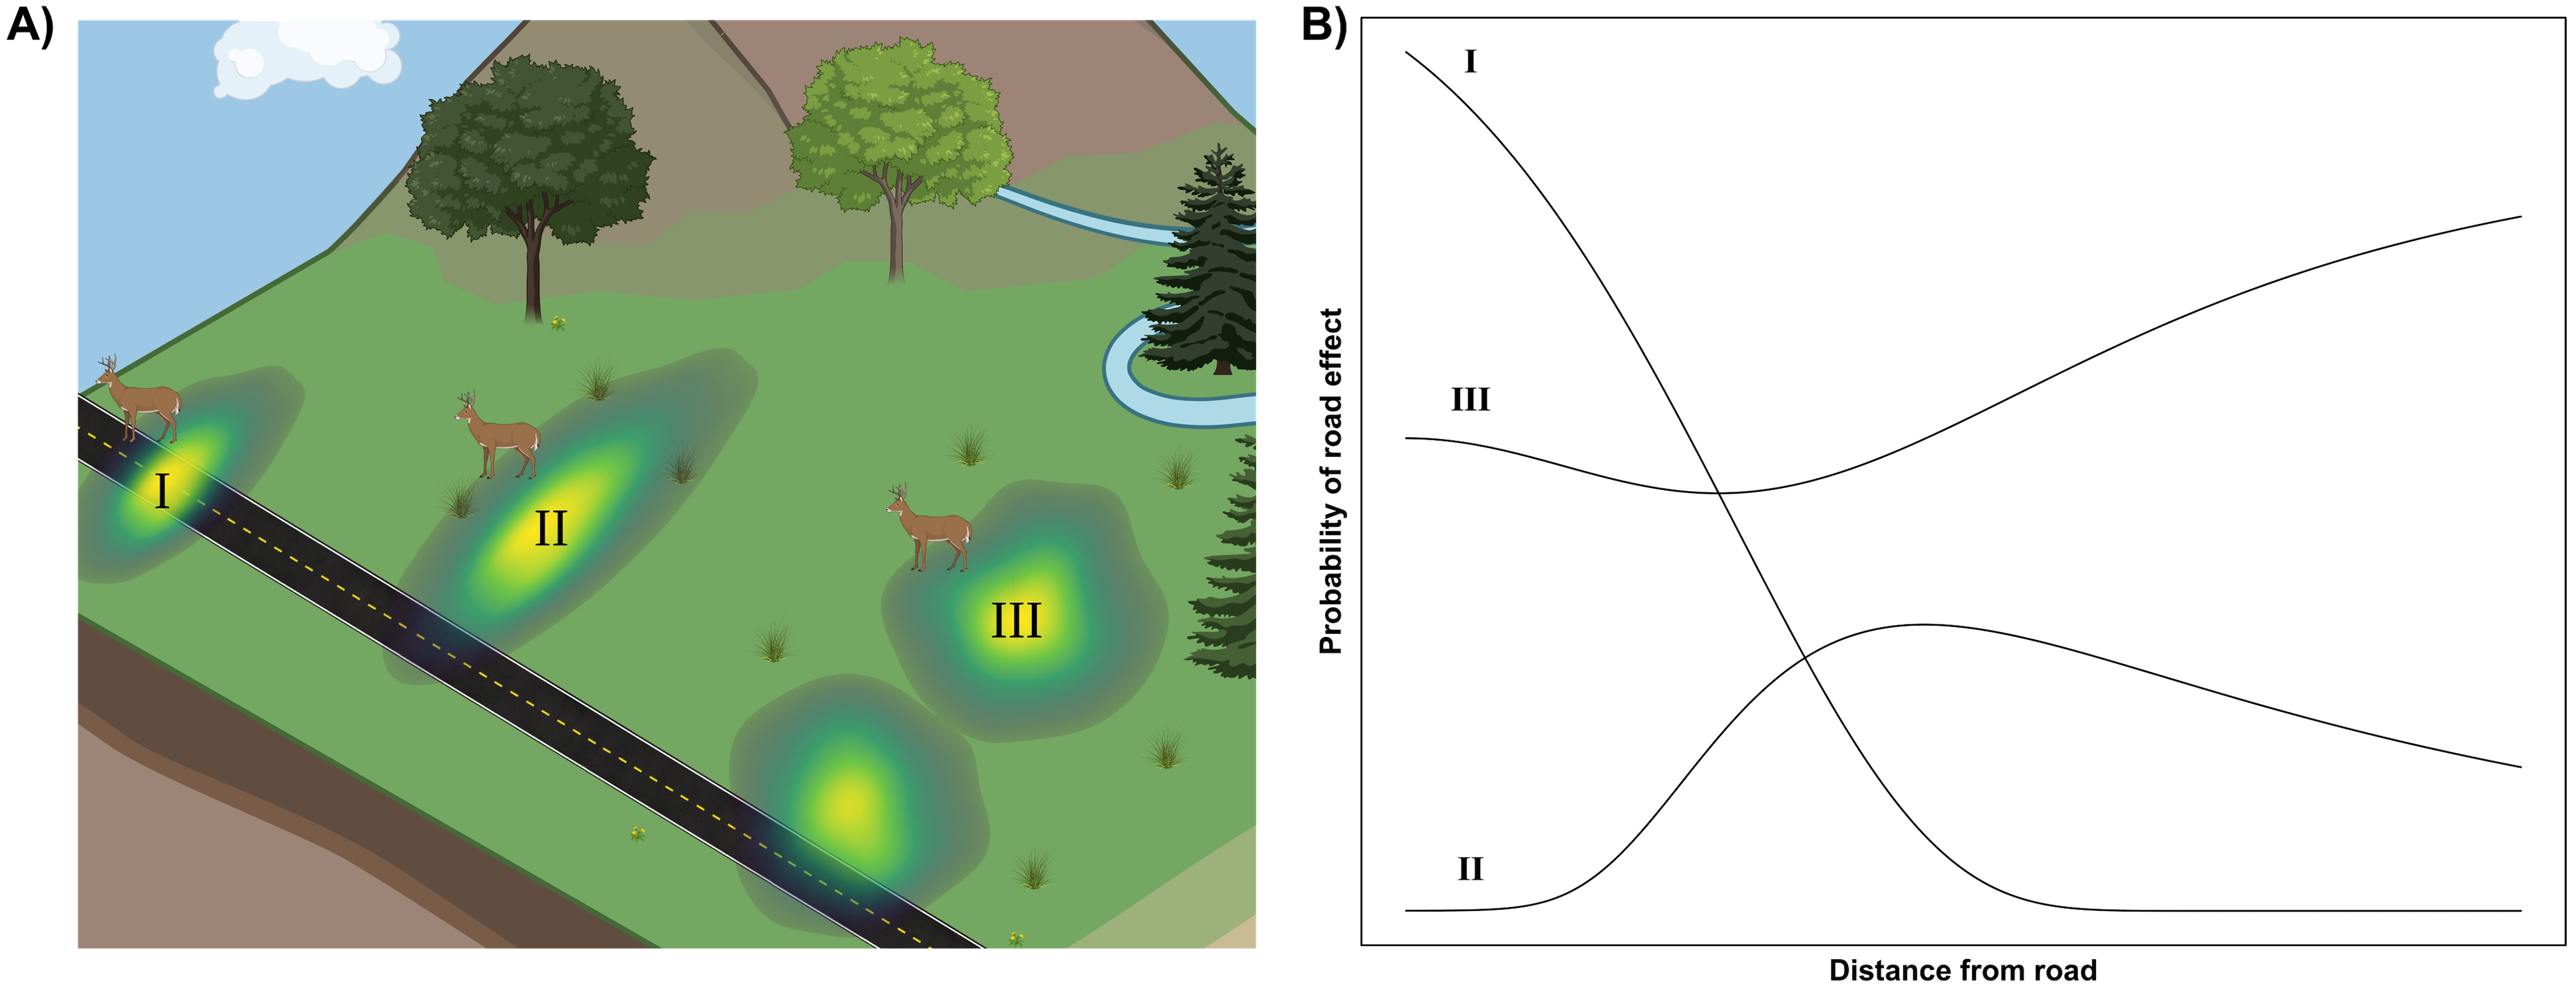
\includegraphics[scale = 0.9]{Theory_Fig}
\caption{Theoretical depiction of the probabilistic road effect (PRE). Panel A shows three animal home ranges that vary in extent and overlap with a road. Animal I has a small home range with high road overlap, Animal II has a small home range with low road overlap, and Animal III has a large home range with intermediate overlap. Note how the three different patterns of space use shown in A result in different PREs in B. As more home range area overlaps with roads, the probability of a road mortality increases, thereby increasing the probability of a road effect occurring. Similarly, as an animal’s home range increases, its ecological effects become more diffuse and the effects of a road mortality may be felt over a larger area. Panel A was created with BioRender.}
\label{Fig:PRE}
\end{figure}


% ----------------------------------------------------------------
% The Probabilistic Road Effect for Giant Anteaters
% ----------------------------------------------------------------

\section*{The Probabilistic Road Effect for Giant Anteaters}

Here, we demonstrate the utility of a probabilistic representation of the road effect on a pair of giant anteaters (\textit{Myrmecophaga tridactyla}) from the Brazilian Cerrado. Giant anteaters are the largest extant anteater, reaching over 2m and weighing up to 50kg \citep{McNab:1984} and are distributed throughout Central and South America \citep{Gardner:2008}. Giant anteater populations have suffered severe reductions and wildlife-vehicle-collisions are a major threat to their survival \citep{Ascensao:2021, Noonan:2022b}. Wild giant anteaters were captured between 2017 and 2018, in the vicinity of the three paved highways in the state of Mato Grosso do Sul, in the Cerrado biome, and equipped with tracking collars that obtained GPS fixes at 20-min intervals \citep[for full details see][]{Noonan:2022b}. A preliminary analysis on these data suggested that these individuals occupied fixed home ranges that regularly overlap paved highways. Following the workflow described above, we estimated the PRE for these two individuals in \texttt{R} \citep[ver. 4.2.1,][]{RAlanguageanden:2016wf}. Home range areas were estimated using Autocorrelated Kernel Density Estimation \citep[AKDE,][]{Fleming:2015tw} via the \texttt{ctmm R} package \citep[ver. 1.1.0,][]{Calabrese:2016ey}. 

\begin{figure}[h!]
\centering
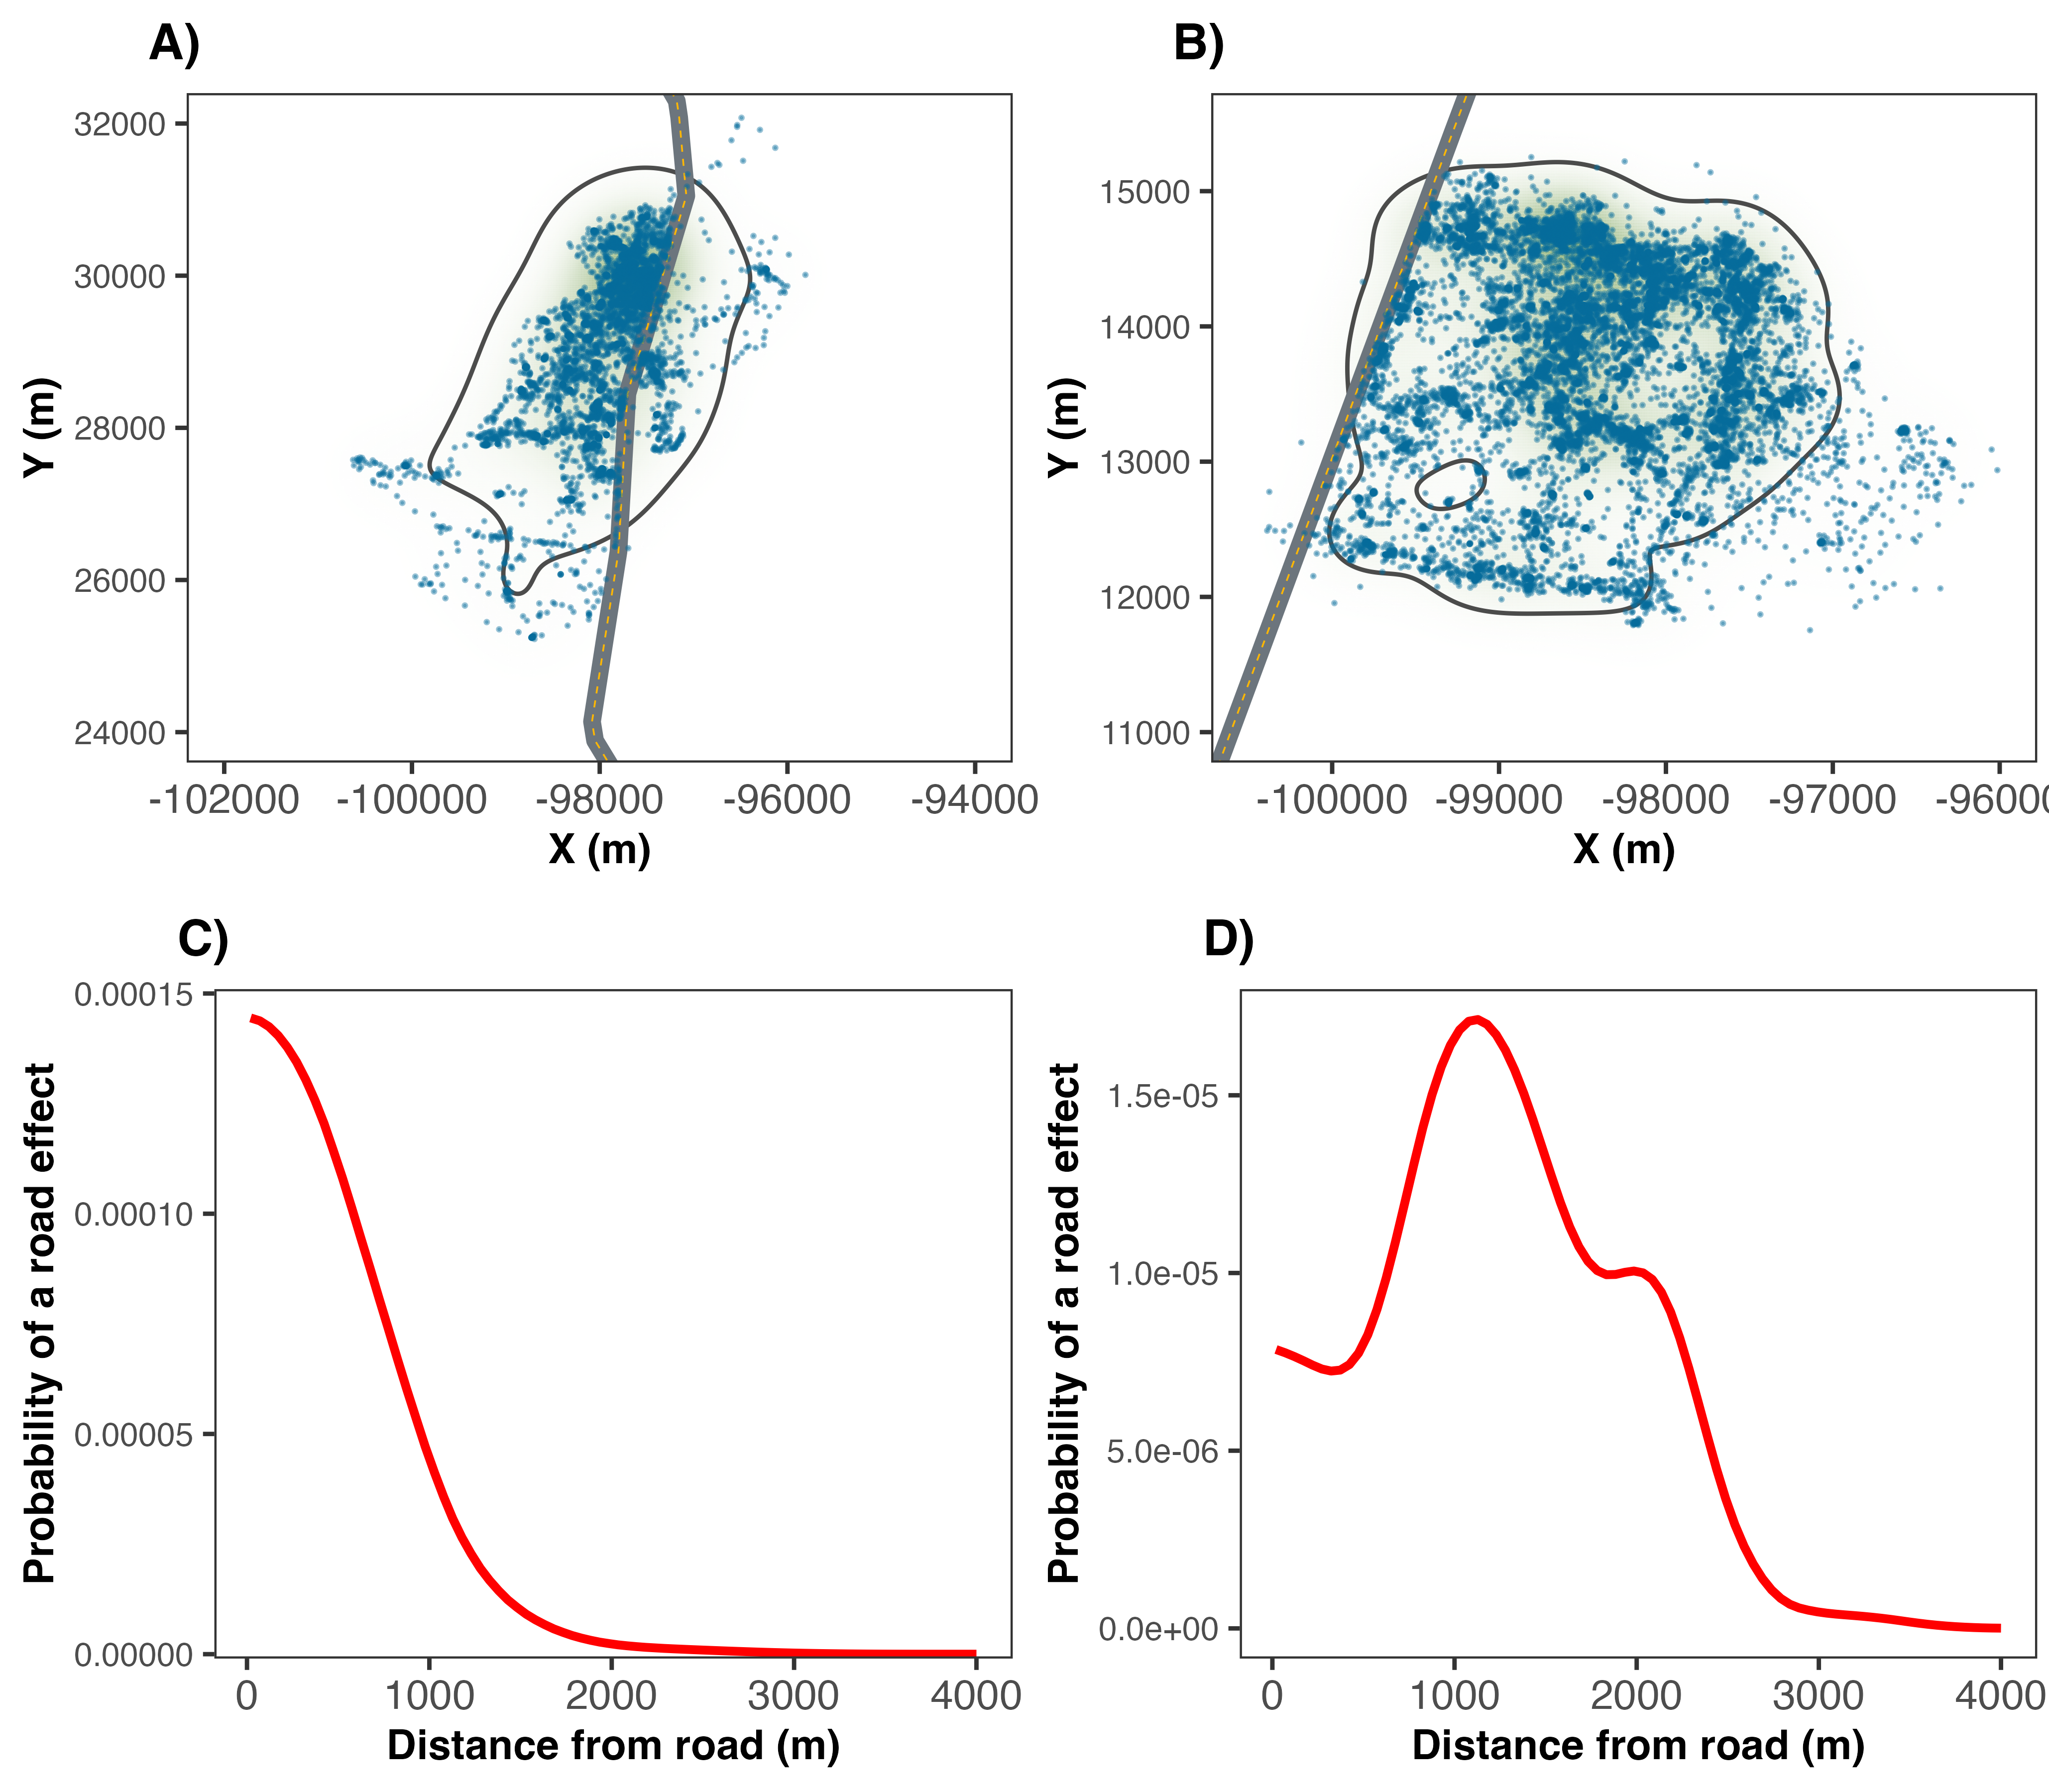
\includegraphics[scale= 0.9]{Anteater_RE}
\caption{The relationship between space use and the road effect zone for two giant anteaters in the Brazilian Cerrado. Note how in panel A), the animal lives right along the roadside, so the ecological effects of a road mortality are greatest near the road, as shown in panel C). In Panel B), the animal's home range was further from the road and while the overall road effect was weaker, it peaked between 1-2km from the road.}
\label{Fig:anteaters}
\end{figure}

The two animals we estimated PREs for exhibited two different patterns in space use. One animal occupied a home range that was centered on the road (Fig.~\ref{Fig:anteaters}A), whereas the other occupied the roadside and surrounding area, but spent little time on the road itself (Fig.~\ref{Fig:anteaters}B). As would be expected for the animal that lived right along the roadside, the ecological effects of a road mortality were greatest near the road (Fig.~\ref{Fig:anteaters}C). For the second animal, their home range was further from the road, resulting in a weaker overall road effect, but one that peaked in probability between 1-2km from the road (Fig.~\ref{Fig:anteaters}D). In other words, although $P\{\mathrm{Roadkilled}\}$ was greater for the first giant anteater, the road has the probability to impact the ecosystem more than 2km away from the road through the loss of the second giant anteater.


% ----------------------------------------------------------------
% Discussion
% ----------------------------------------------------------------


\section*{Discussion}

The idea that ecological conditions will be more pristine the further one moves from away from a road has been a focal point of road ecology research since \cite{Forman:1998} first introduced the concept of the Road Effect Zone more than two decades ago \citep{Reijnen:1996, Forman:1998, Forman:2000b, Semlitsch:2007, Eigenbrod:2009, Peaden:2015, Brady:2017, Andrasi:2021}. This conventional REZ focuses on quantifying the area over which roads alter measurable ecological impacts, typically community composition or population densities \citep{Reijnen:1996, Truscott:2005, Fahrig:2009, Andrasi:2021}. While this concept has proven informative for understanding the ecological footprint of roads, the static nature of the REZ means that impacts related to animal movement and species interactions are not captured. For instance, consider a situation where there is a measurable reduction in the population density of a species near a road. This effect may be due to increased road-induced mortality, but it may also be due to road-avoidance and altered movement. Each of these mechanisms may reduce roadside population densities, but each would have different ecological impacts and require different mitigation strategies. Here we demonstrate how probability theory can provide a powerful tool for re-thinking the road effect zone, and an individual-based framework for scaling up to population-, or community-level effects.

Of note is the fact that our PRE framework as defined here relies on the assumption that an animal's probability of being road-killed is directly proportional to the time it spends on a road. This is clearly an overly simplistic assumption as factors such as traffic volume and learning will impact mortality rates \citep{Mumme:2000, van:2005, Ford:2007, Noonan:2022b, Ascensao:2022}. Nonetheless, because our framework is based on quantifying the joint probability of independent events, incorporating additional information affecting $P\{\mathrm{Roadkilled}\}$ is straightforward. Indeed, this flexibility is one of the strengths of this framework. For instance, if signage (e.g., altered speed limits, wildlife corridor notices, etc.) is being considered as a mortality reduction strategy, the effect should be a measureable reduction in $P\{\mathrm{Roadkilled}\}$, and, consequently, $P\{\mathrm{Road~Effect}\}$. Similarly, if a practitioner is tasked with making recommendations on the placement of a road-crossing structure, the conventional REZ would suggest that the effects of reduced road mortality will be felt according to some decay function as shown in figure~\ref{Fig:REZ}. In reality, however, the capacity for animals to move freely across a roadway with $P\{\mathrm{Roadkilled}\} = 0$ (i.e., the benefit provided by the crossing structure) can have ecosystem-wide benefits over vastly larger distances than the conventional REZ might suggest, depending on the vagility and behaviour of the animals the crossing-structure would benefit. The PRE thus provides ecologists and conservation practitioners with a dynamic metric for quantifying the ecosystem-wide impacts of roads, and/or the benefits of management strategies.

In this study, we have developed a framework for estimating road effect zones from animal movement data. Using movement data from giant anteaters occupying roadside habitats in Brazil, we have demonstrated how this framework can be used in practice to understand the ecological impacts of a road, and help inform species management. Notably, this framework builds straightforwardly off of home-range estimation and requires no specialized data collection protocols, allowing researchers to easily quantify the potential ecological impacts of roads for a variety of taxa.

% ----------------------------------------------------------------
% Acknowledgments
% ----------------------------------------------------------------

%\section*{Acknowledgments}
%
%This work was supported by an NSERC Discovery Grant RGPIN-2021-02758 to MJN, as well as the Canadian Foundation for Innovation. We would like to thank the donors to the Anteaters and Highways Project especially the Foundation Segre as well as North American and European Zoos listed at \url{http://www.giantanteater.org/}. We would also like to thank the owners of all the ranches that allowed us to monitor animals on their property, in particular Nhuveira, Quatro Irmãos and Santa Lourdes ranches and also thank to M. Alves, D. Kluyber, C. Luba, A. Alves, as well as all of the volunteers who assisted in carrying out the fieldwork.

% ----------------------------------------------------------------
% Statement of Authorship
% ----------------------------------------------------------------

%\section*{Statement of Authorship}
%
%MJN and ATF conceived the study, collected the data, and wrote the original draft.
%ALJD provided the tracking data.
%MJN oversaw data analysis and developed the code. 
%All authors reviewed and edited the writing at all stages of revision.
%
%\section*{Data and Code Availability}
%
%The \texttt{R} scripts required to reproduce these analyses and estimate the PRE from animal tracking data are openly available at \url{https://github.com/NoonanM/Road_Effect_Zone}. The Giant anteater tracking data are openly available on MoveBank (MoveBank ID: 1574830796).


% ----------------------------------------------------------------
% Bibliography
% ----------------------------------------------------------------
% You can either type your references following the examples below, or
% compile your BiBTeX database and paste the contents of your .bbl file
% here. The amnatnat.bst style file should work for this---but please
% let us know if you run into any hitches with it!
%
% If you upload a .bib file with your submission, please upload the .bbl
% file as well; this will be required for typesetting.
%
% The list below includes sample journal articles, book chapters, and
% Dryad references.

%\bibliography{Refs}

\begin{thebibliography}{40}
\providecommand{\natexlab}[1]{#1}

\bibitem[{Andrasi et~al.(2021)Andrasi, Jaeger, Heinicke, Metcalfe, and
  Hockings}]{Andrasi:2021}
Andrasi, B., J.~A. Jaeger, S.~Heinicke, K.~Metcalfe, and K.~J. Hockings. 2021.
\newblock Quantifying the road-effect zone for a critically endangered primate.
\newblock Conservation Letters 14:e12839.

\bibitem[{Ascens{\~a}o and Desbiez(2022)}]{Ascensao:2022}
Ascens{\~a}o, F., and A.~L. Desbiez. 2022.
\newblock Assessing the impact of roadkill on the persistence of wildlife
  populations: a case study on the giant anteater.
\newblock bioRxiv .

\bibitem[{Ascens{\~a}o et~al.(2021)Ascens{\~a}o, Yogui, Alves, Alves, Abra, and
  Desbiez}]{Ascensao:2021}
Ascens{\~a}o, F., D.~R. Yogui, M.~H. Alves, A.~C. Alves, F.~Abra, and A.~L.
  Desbiez. 2021.
\newblock Preventing wildlife roadkill can offset mitigation investments in
  short-medium term.
\newblock Biological Conservation 253:108902.

\bibitem[{Augustine and McNaughton(1998)}]{Augustine:1998}
Augustine, D.~J., and S.~J. McNaughton. 1998.
\newblock Ungulate effects on the functional species composition of plant
  communities: herbivore selectivity and plant tolerance.
\newblock The Journal of wildlife management pages 1165--1183.

\bibitem[{Biel{\v{c}}ik et~al.(2019)Biel{\v{c}}ik, Aguilar-Trigueros, Lakovic,
  Jeltsch, and Rillig}]{Bielvcik:2019}
Biel{\v{c}}ik, M., C.~A. Aguilar-Trigueros, M.~Lakovic, F.~Jeltsch, and M.~C.
  Rillig. 2019.
\newblock The role of active movement in fungal ecology and community assembly.
\newblock Movement ecology 7:1--12.

\bibitem[{Brady and Richardson(2017)}]{Brady:2017}
Brady, S.~P., and J.~L. Richardson. 2017.
\newblock Road ecology: shifting gears toward evolutionary perspectives.
\newblock Frontiers in Ecology and the Environment 15:91--98.

\bibitem[{Brown and Brown(2013)}]{Brown:2013}
Brown, C.~R., and M.~B. Brown. 2013.
\newblock Where has all the road kill gone?
\newblock Current Biology 23:R233--R234.

\bibitem[{Burt(1943)}]{Burt:1943he}
Burt, W.~H. 1943.
\newblock {Territoriality and Home Range Concepts as Applied to Mammals}.
\newblock Journal of Mammalogy 24:346--352.

\bibitem[{Calabrese et~al.(2016)Calabrese, Fleming, and
  Gurarie}]{Calabrese:2016ey}
Calabrese, J.~M., C.~H. Fleming, and E.~Gurarie. 2016.
\newblock ctmm: an {R} package for analyzing animal relocation data as a
  continuous-time stochastic process.
\newblock Methods in Ecology and Evolution 7:1124--1132.

\bibitem[{Carter et~al.(2020)Carter, Killion, Easter, Brandt, and
  Ford}]{Carter:2020}
Carter, N., A.~Killion, T.~Easter, J.~Brandt, and A.~Ford. 2020.
\newblock Road development in asia: Assessing the range-wide risks to tigers.
\newblock Science Advances 6:eaaz9619.

\bibitem[{Coffin(2007)}]{Coffin:2007}
Coffin, A.~W. 2007.
\newblock From roadkill to road ecology: a review of the ecological effects of
  roads.
\newblock Journal of transport Geography 15:396--406.

\bibitem[{Desbiez et~al.(2020)Desbiez, Bertassoni, and
  Traylor-Holzer}]{Desbiez:2020}
Desbiez, A. L.~J., A.~Bertassoni, and K.~Traylor-Holzer. 2020.
\newblock Population viability analysis as a tool for giant anteater
  conservation.
\newblock Perspectives in Ecology and Conservation 18:124--131.

\bibitem[{Eigenbrod et~al.(2009)Eigenbrod, Hecnar, and Fahrig}]{Eigenbrod:2009}
Eigenbrod, F., S.~J. Hecnar, and L.~Fahrig. 2009.
\newblock Quantifying the road-effect zone: threshold effects of a motorway on
  anuran populations in ontario, canada.
\newblock Ecology and Society 14.

\bibitem[{Fahrig and Rytwinski(2009)}]{Fahrig:2009}
Fahrig, L., and T.~Rytwinski. 2009.
\newblock Effects of roads on animal abundance: an empirical review and
  synthesis.
\newblock Ecology and society 14.

\bibitem[{Fleming et~al.(2015)Fleming, Fagan, Mueller, Olson, Leimgruber, and
  Calabrese}]{Fleming:2015tw}
Fleming, C.~H., W.~F. Fagan, T.~Mueller, K.~A. Olson, P.~Leimgruber, and J.~M.
  Calabrese. 2015.
\newblock {Rigorous home range estimation with movement data: a new
  autocorrelated kernel density estimator.}
\newblock Ecology 96:1182--1188.

\bibitem[{Ford and Fahrig(2007)}]{Ford:2007}
Ford, A.~T., and L.~Fahrig. 2007.
\newblock Diet and body size of north american mammal road mortalities.
\newblock Transportation Research Part D: Transport and Environment
  12:498--505.

\bibitem[{Ford et~al.(2020)Ford, Sunter, Fauvelle, Bradshaw, Ford, Hutchen,
  Phillipow, and Teichman}]{Ford:2020}
Ford, A.~T., E.~J. Sunter, C.~Fauvelle, J.~L. Bradshaw, B.~Ford, J.~Hutchen,
  N.~Phillipow, and K.~J. Teichman. 2020.
\newblock Effective corridor width: linking the spatial ecology of wildlife
  with land use policy.
\newblock European Journal of Wildlife Research 66:1--10.

\bibitem[{Forman(2000)}]{Forman:2000}
Forman, R.~T. 2000.
\newblock Estimate of the area affected ecologically by the road system in the
  united states.
\newblock Conservation biology 14:31--35.

\bibitem[{Forman and Alexander(1998)}]{Forman:1998}
Forman, R.~T., and L.~E. Alexander. 1998.
\newblock Roads and their major ecological effects.
\newblock Annual review of ecology and systematics 29:207--231.

\bibitem[{Forman and Deblinger(2000)}]{Forman:2000b}
Forman, R.~T., and R.~D. Deblinger. 2000.
\newblock The ecological road-effect zone of a massachusetts (usa) suburban
  highway.
\newblock Conservation biology 14:36--46.

\bibitem[{Forman et~al.(2003)Forman, Sperling, Bissonette, Clevenger, Cutshall,
  Dale, Fahrig, France, Goldman, Heanue et~al.}]{Forman:2003}
Forman, R.~T., D.~Sperling, J.~A. Bissonette, A.~P. Clevenger, C.~D. Cutshall,
  V.~H. Dale, L.~Fahrig, R.~L. France, C.~R. Goldman, K.~Heanue, et~al. 2003.
\newblock Road ecology: science and solutions.
\newblock Island press.

\bibitem[{Gardner(2008)}]{Gardner:2008}
Gardner, A.~L. 2008.
\newblock Mammals of South America, volume 1: marsupials, xenarthrans, shrews,
  and bats, vol.~2.
\newblock University of Chicago Press.

\bibitem[{Ibisch et~al.(2016)Ibisch, Hoffmann, Kreft, Pe'er, Kati,
  Biber-Freudenberger, DellaSala, Vale, Hobson, and Selva}]{Ibisch:2016}
Ibisch, P.~L., M.~T. Hoffmann, S.~Kreft, G.~Pe'er, V.~Kati,
  L.~Biber-Freudenberger, D.~A. DellaSala, M.~M. Vale, P.~R. Hobson, and
  N.~Selva. 2016.
\newblock A global map of roadless areas and their conservation status.
\newblock Science 354:1423--1427.

\bibitem[{Kauffman et~al.(2020)Kauffman, Copeland, Berg, Bergen, Cole,
  Cuzzocreo, Dewey, Fattebert, Gagnon, Gelzer et~al.}]{Kauffman:2020}
Kauffman, M., H.~Copeland, J.~Berg, S.~Bergen, E.~Cole, M.~Cuzzocreo, S.~Dewey,
  J.~Fattebert, J.~Gagnon, E.~Gelzer, et~al. 2020.
\newblock Ungulate migrations of the western united states, volume 1.
\newblock Tech. rep., US Geological Survey.

\bibitem[{Kauffman et~al.(2021)Kauffman, Cagnacci, Chamaill{\'e}-Jammes,
  Hebblewhite, Hopcraft, Merkle, Mueller, Mysterud, Peters, Roettger
  et~al.}]{Kauffman:2021}
Kauffman, M.~J., F.~Cagnacci, S.~Chamaill{\'e}-Jammes, M.~Hebblewhite, J.~G.~C.
  Hopcraft, J.~A. Merkle, T.~Mueller, A.~Mysterud, W.~Peters, C.~Roettger,
  et~al. 2021.
\newblock Mapping out a future for ungulate migrations.
\newblock Science 372:566--569.

\bibitem[{Kie et~al.(2010)Kie, Matthiopoulos, Fieberg, Powell, Cagnacci,
  Mitchell, Gaillard, and Moorcroft}]{Kie:2010es}
Kie, J.~G., J.~Matthiopoulos, J.~Fieberg, R.~A. Powell, F.~Cagnacci, M.~S.
  Mitchell, J.-M. Gaillard, and P.~R. Moorcroft. 2010.
\newblock {The home-range concept: are traditional estimators still relevant
  with modern telemetry technology?}
\newblock Philosophical Transactions of the Royal Society of London. Series B:
  Biological Sciences 365:2221--2231.

\bibitem[{McNab(1984)}]{McNab:1984}
McNab, B.~K. 1984.
\newblock Physiological convergence amongst ant-eating and termite-eating
  mammals.
\newblock Journal of Zoology 203:485--510.

\bibitem[{Mumme et~al.(2000)Mumme, Schoech, Woolfenden, and
  Fitzpatrick}]{Mumme:2000}
Mumme, R.~L., S.~J. Schoech, G.~E. Woolfenden, and J.~W. Fitzpatrick. 2000.
\newblock Life and death in the fast lane: Demographic consequences of road
  mortality in the florida scrub-jay.
\newblock Conservation biology 14:501--512.

\bibitem[{Noonan et~al.(2022)Noonan, Ascens{\~a}o, Yogui, and
  Desbiez}]{Noonan:2022b}
Noonan, M.~J., F.~Ascens{\~a}o, D.~R. Yogui, and A.~L. Desbiez. 2022.
\newblock Roads as ecological traps for giant anteaters.
\newblock Animal Conservation 25:182--194.

\bibitem[{Noonan et~al.(2019)Noonan, Tucker, Fleming, Akre, Alberts, Ali,
  Altmann, Antunes, Belant, Beyer, Blaum, B{\"o}hning-Gaese, Cullen~Jr,
  de~Paula, Dekker, Drescher-Lehman, Farwig, Fichtel, Fischer, Ford, Goheen,
  Janssen, Jeltsch, Kauffman, Kappeler, Koch, LaPoint, Catherine~Markham,
  Medici, Morato, Nathan, Oliveira-Santos, Olson, Patterson, Paviolo, Ramalho,
  Roesner, Schabo, Selva, Sergiel, Xavier~da Silva, Spiegel, Thompson, Ullmann,
  Zi{\c e}ba, Zwijacz-Kozica, Fagan, Mueller, and Calabrese}]{AKDEvsKDE}
Noonan, M.~J., M.~A. Tucker, C.~H. Fleming, T.~Akre, S.~C. Alberts, A.~H. Ali,
  J.~Altmann, P.~C. Antunes, J.~L. Belant, D.~Beyer, N.~Blaum,
  K.~B{\"o}hning-Gaese, L.~Cullen~Jr, R.~C. de~Paula, J.~Dekker,
  J.~Drescher-Lehman, N.~Farwig, C.~Fichtel, C.~Fischer, A.~Ford, J.~R. Goheen,
  R.~Janssen, F.~Jeltsch, M.~Kauffman, P.~M. Kappeler, F.~Koch, S.~LaPoint,
  A.~Catherine~Markham, E.~P. Medici, R.~G. Morato, R.~Nathan, L.~G.~R.
  Oliveira-Santos, K.~A. Olson, B.~D. Patterson, A.~Paviolo, E.~E. Ramalho,
  S.~Roesner, D.~Schabo, N.~Selva, A.~Sergiel, M.~Xavier~da Silva, O.~Spiegel,
  P.~Thompson, W.~Ullmann, F.~Zi{\c e}ba, T.~Zwijacz-Kozica, W.~F. Fagan,
  T.~Mueller, and J.~M. Calabrese. 2019.
\newblock A comprehensive analysis of autocorrelation and bias in home range
  estimation.
\newblock Ecological Monographs 0:e01344.

\bibitem[{Peaden et~al.(2015)Peaden, Tuberville, Buhlmann, Nafus, and
  Todd}]{Peaden:2015}
Peaden, J.~M., T.~D. Tuberville, K.~A. Buhlmann, M.~G. Nafus, and B.~D. Todd.
  2015.
\newblock Delimiting road-effect zones for threatened species: implications for
  mitigation fencing.
\newblock Wildlife Research 42:650--659.

\bibitem[{{R Core Team}(2016)}]{RAlanguageanden:2016wf}
{R Core Team}. 2016.
\newblock R: A language and environment for statistical computing.

\bibitem[{Reijnen et~al.(1996)Reijnen, Foppen, and Meeuwsen}]{Reijnen:1996}
Reijnen, R., R.~Foppen, and H.~Meeuwsen. 1996.
\newblock The effects of traffic on the density of breeding birds in dutch
  agricultural grasslands.
\newblock Biological conservation 75:255--260.

\bibitem[{Semlitsch et~al.(2007)Semlitsch, Ryan, Hamed, Chatfield, Drehman,
  Pekarek, Spath, and Watland}]{Semlitsch:2007}
Semlitsch, R.~D., T.~J. Ryan, K.~Hamed, M.~Chatfield, B.~Drehman, N.~Pekarek,
  M.~Spath, and A.~Watland. 2007.
\newblock Salamander abundance along road edges and within abandoned logging
  roads in appalachian forests.
\newblock Conservation biology 21:159--167.

\bibitem[{Silva et~al.(2020)Silva, Crane, and Savini}]{Silva:2020}
Silva, I., M.~Crane, and T.~Savini. 2020.
\newblock High roadkill rates in the dong phayayen-khao yai world heritage
  site: Conservation implications of a rising threat to wildlife.
\newblock Animal Conservation 23:466--478.

\bibitem[{Subalusky et~al.(2017)Subalusky, Dutton, Rosi, and
  Post}]{Subalusky:2017}
Subalusky, A.~L., C.~L. Dutton, E.~J. Rosi, and D.~M. Post. 2017.
\newblock Annual mass drownings of the serengeti wildebeest migration influence
  nutrient cycling and storage in the mara river.
\newblock Proceedings of the National Academy of Sciences 114:7647--7652.

\bibitem[{Truscott et~al.(2005)Truscott, Palmer, McGowan, Cape, and
  Smart}]{Truscott:2005}
Truscott, A.-M., S.~Palmer, G.~McGowan, J.~Cape, and S.~Smart. 2005.
\newblock Vegetation composition of roadside verges in scotland: the effects of
  nitrogen deposition, disturbance and management.
\newblock Environmental pollution 136:109--118.

\bibitem[{Tucker et~al.(2021)Tucker, Busana, Huijbregts, and
  Ford}]{Tucker:2021}
Tucker, M.~A., M.~Busana, M.~A. Huijbregts, and A.~T. Ford. 2021.
\newblock Human-induced reduction in mammalian movements impacts seed dispersal
  in the tropics.
\newblock Ecography 44:897--906.

\bibitem[{van Langevelde and Jaarsma(2005)}]{van:2005}
van Langevelde, F., and C.~F. Jaarsma. 2005.
\newblock Using traffic flow theory to model traffic mortality in mammals.
\newblock Landscape ecology 19:895--907.

\bibitem[{Walton et~al.(2017)Walton, Mattisson, Linnell, Stien, and
  Odden}]{Walton:2017}
Walton, Z., J.~Mattisson, J.~D. Linnell, A.~Stien, and J.~Odden. 2017.
\newblock The cost of migratory prey: seasonal changes in semi-domestic
  reindeer distribution influences breeding success of eurasian lynx in
  northern norway.
\newblock Oikos 126:642--650.

\end{thebibliography}


\newpage{}

\section*{Figure legends}

\setcounter{figure}{0}


\begin{figure}[h!]
%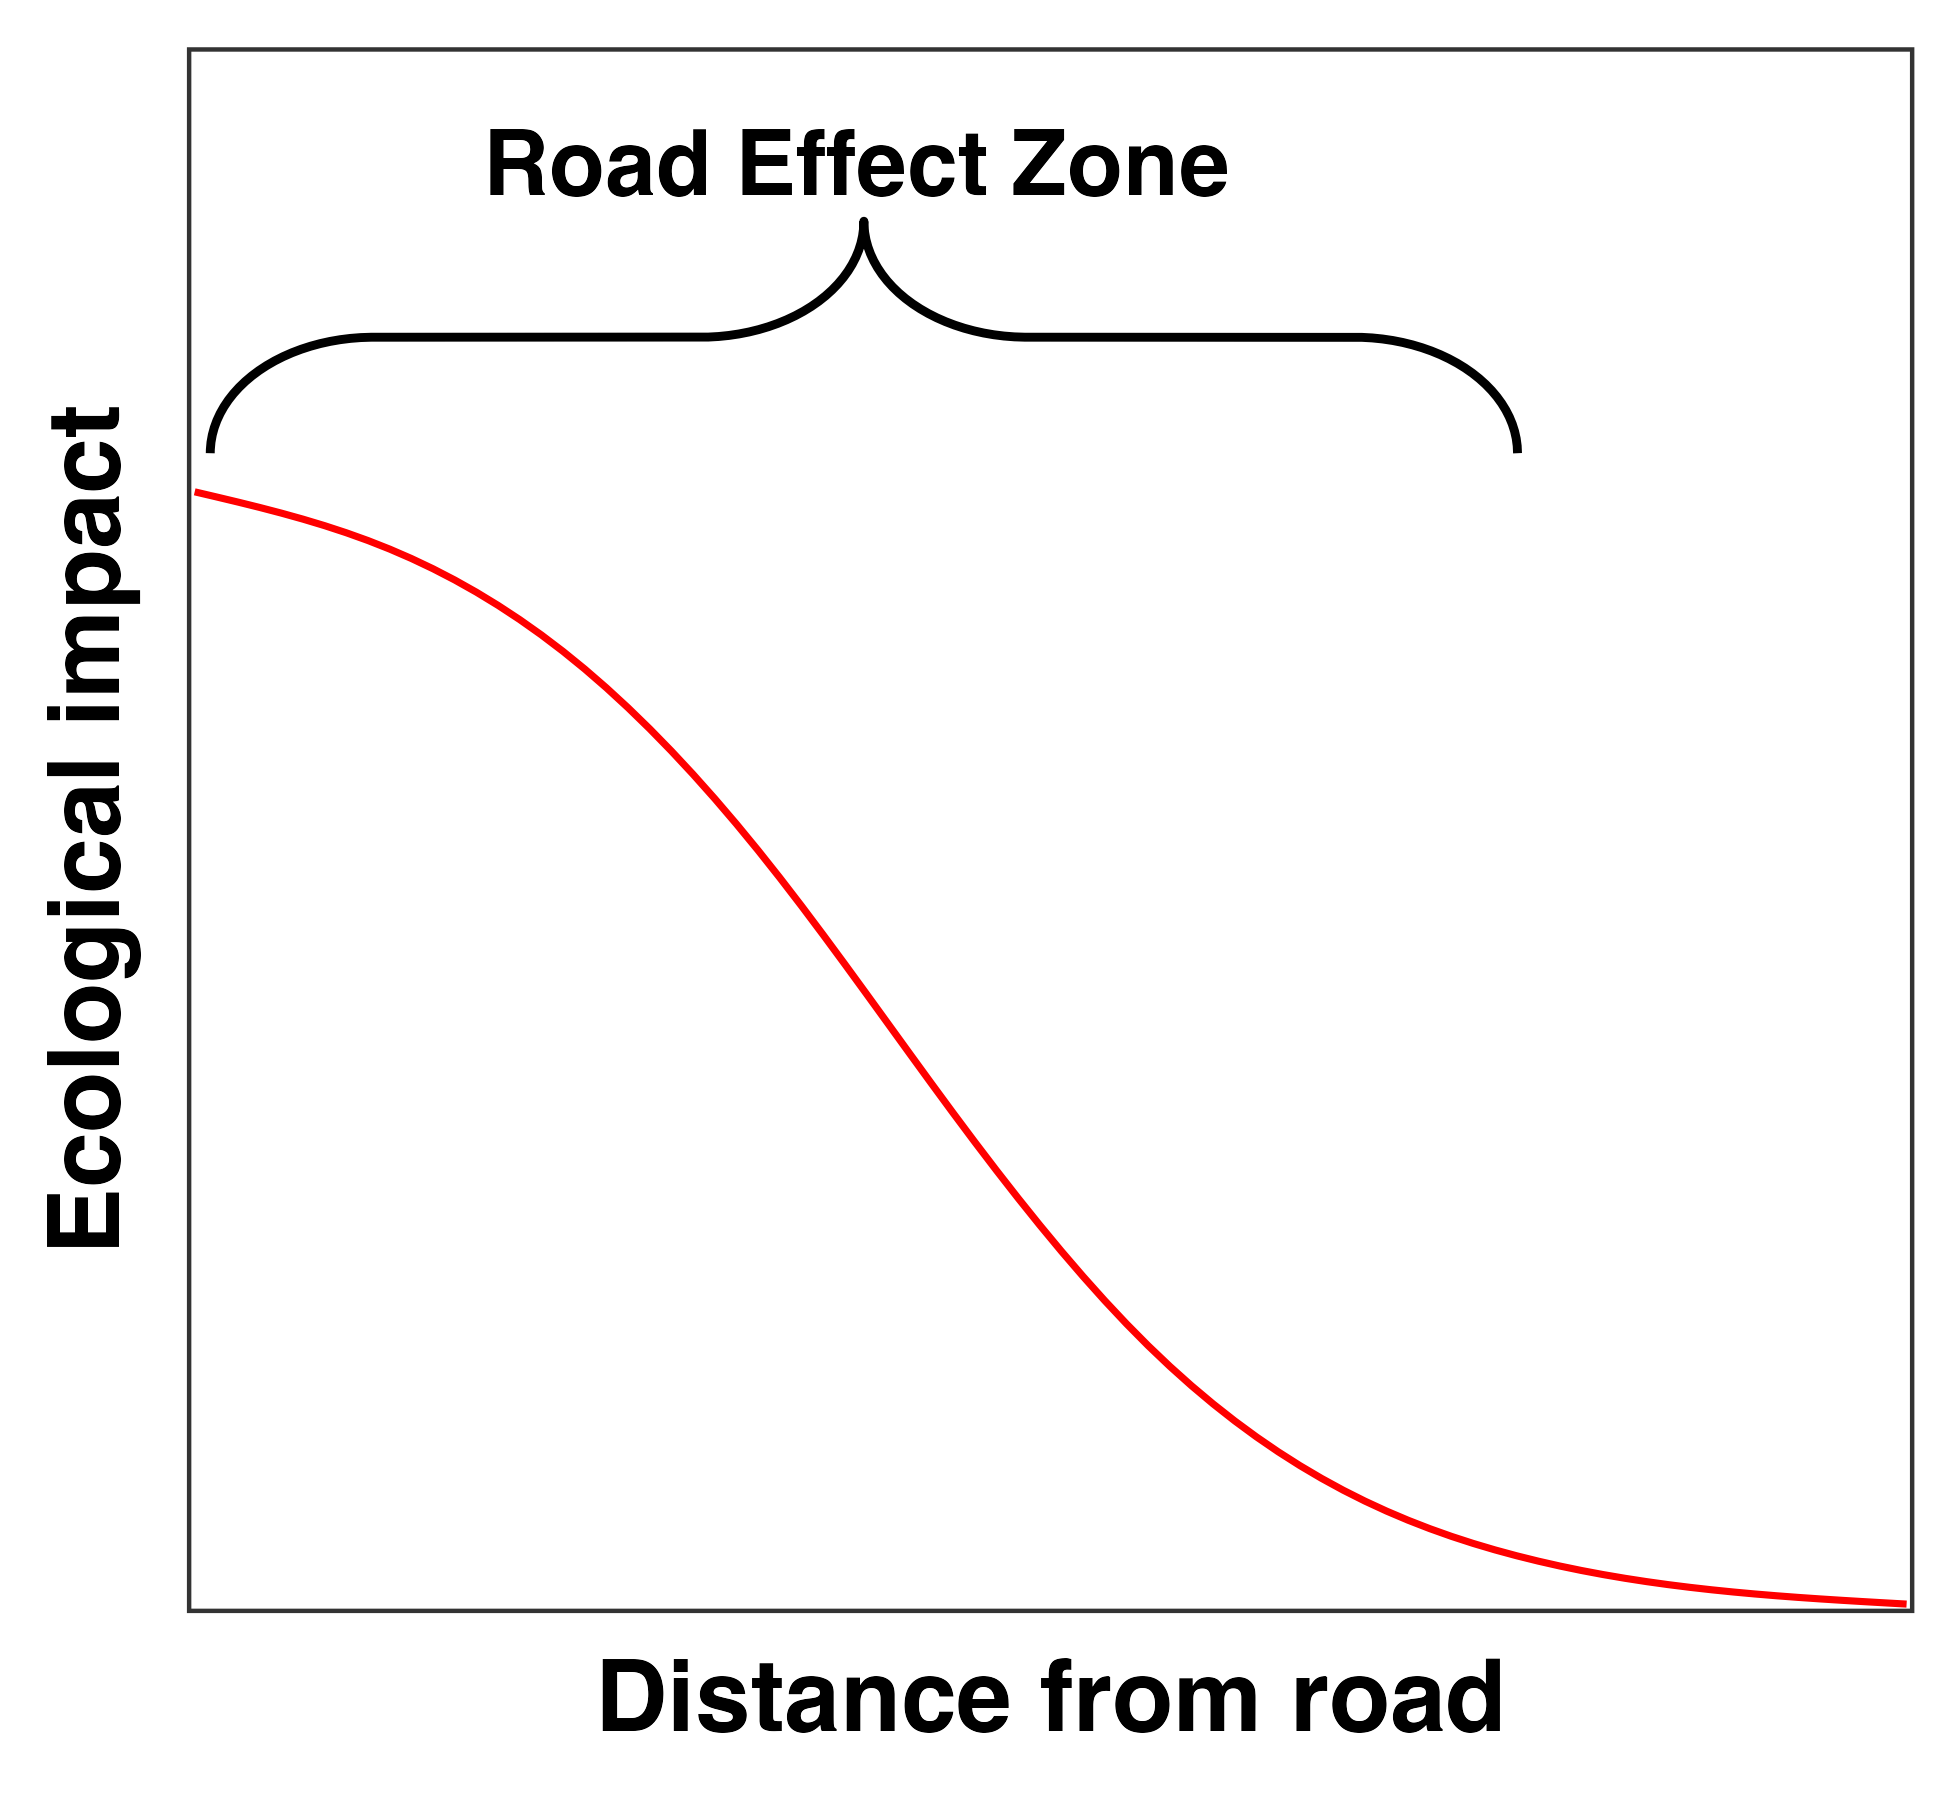
\includegraphics{REZ}
\caption{Theoretical depiction of the road effect zone as originally defined by \cite{Forman:1998}.}
\end{figure}

\begin{figure}[h!]
%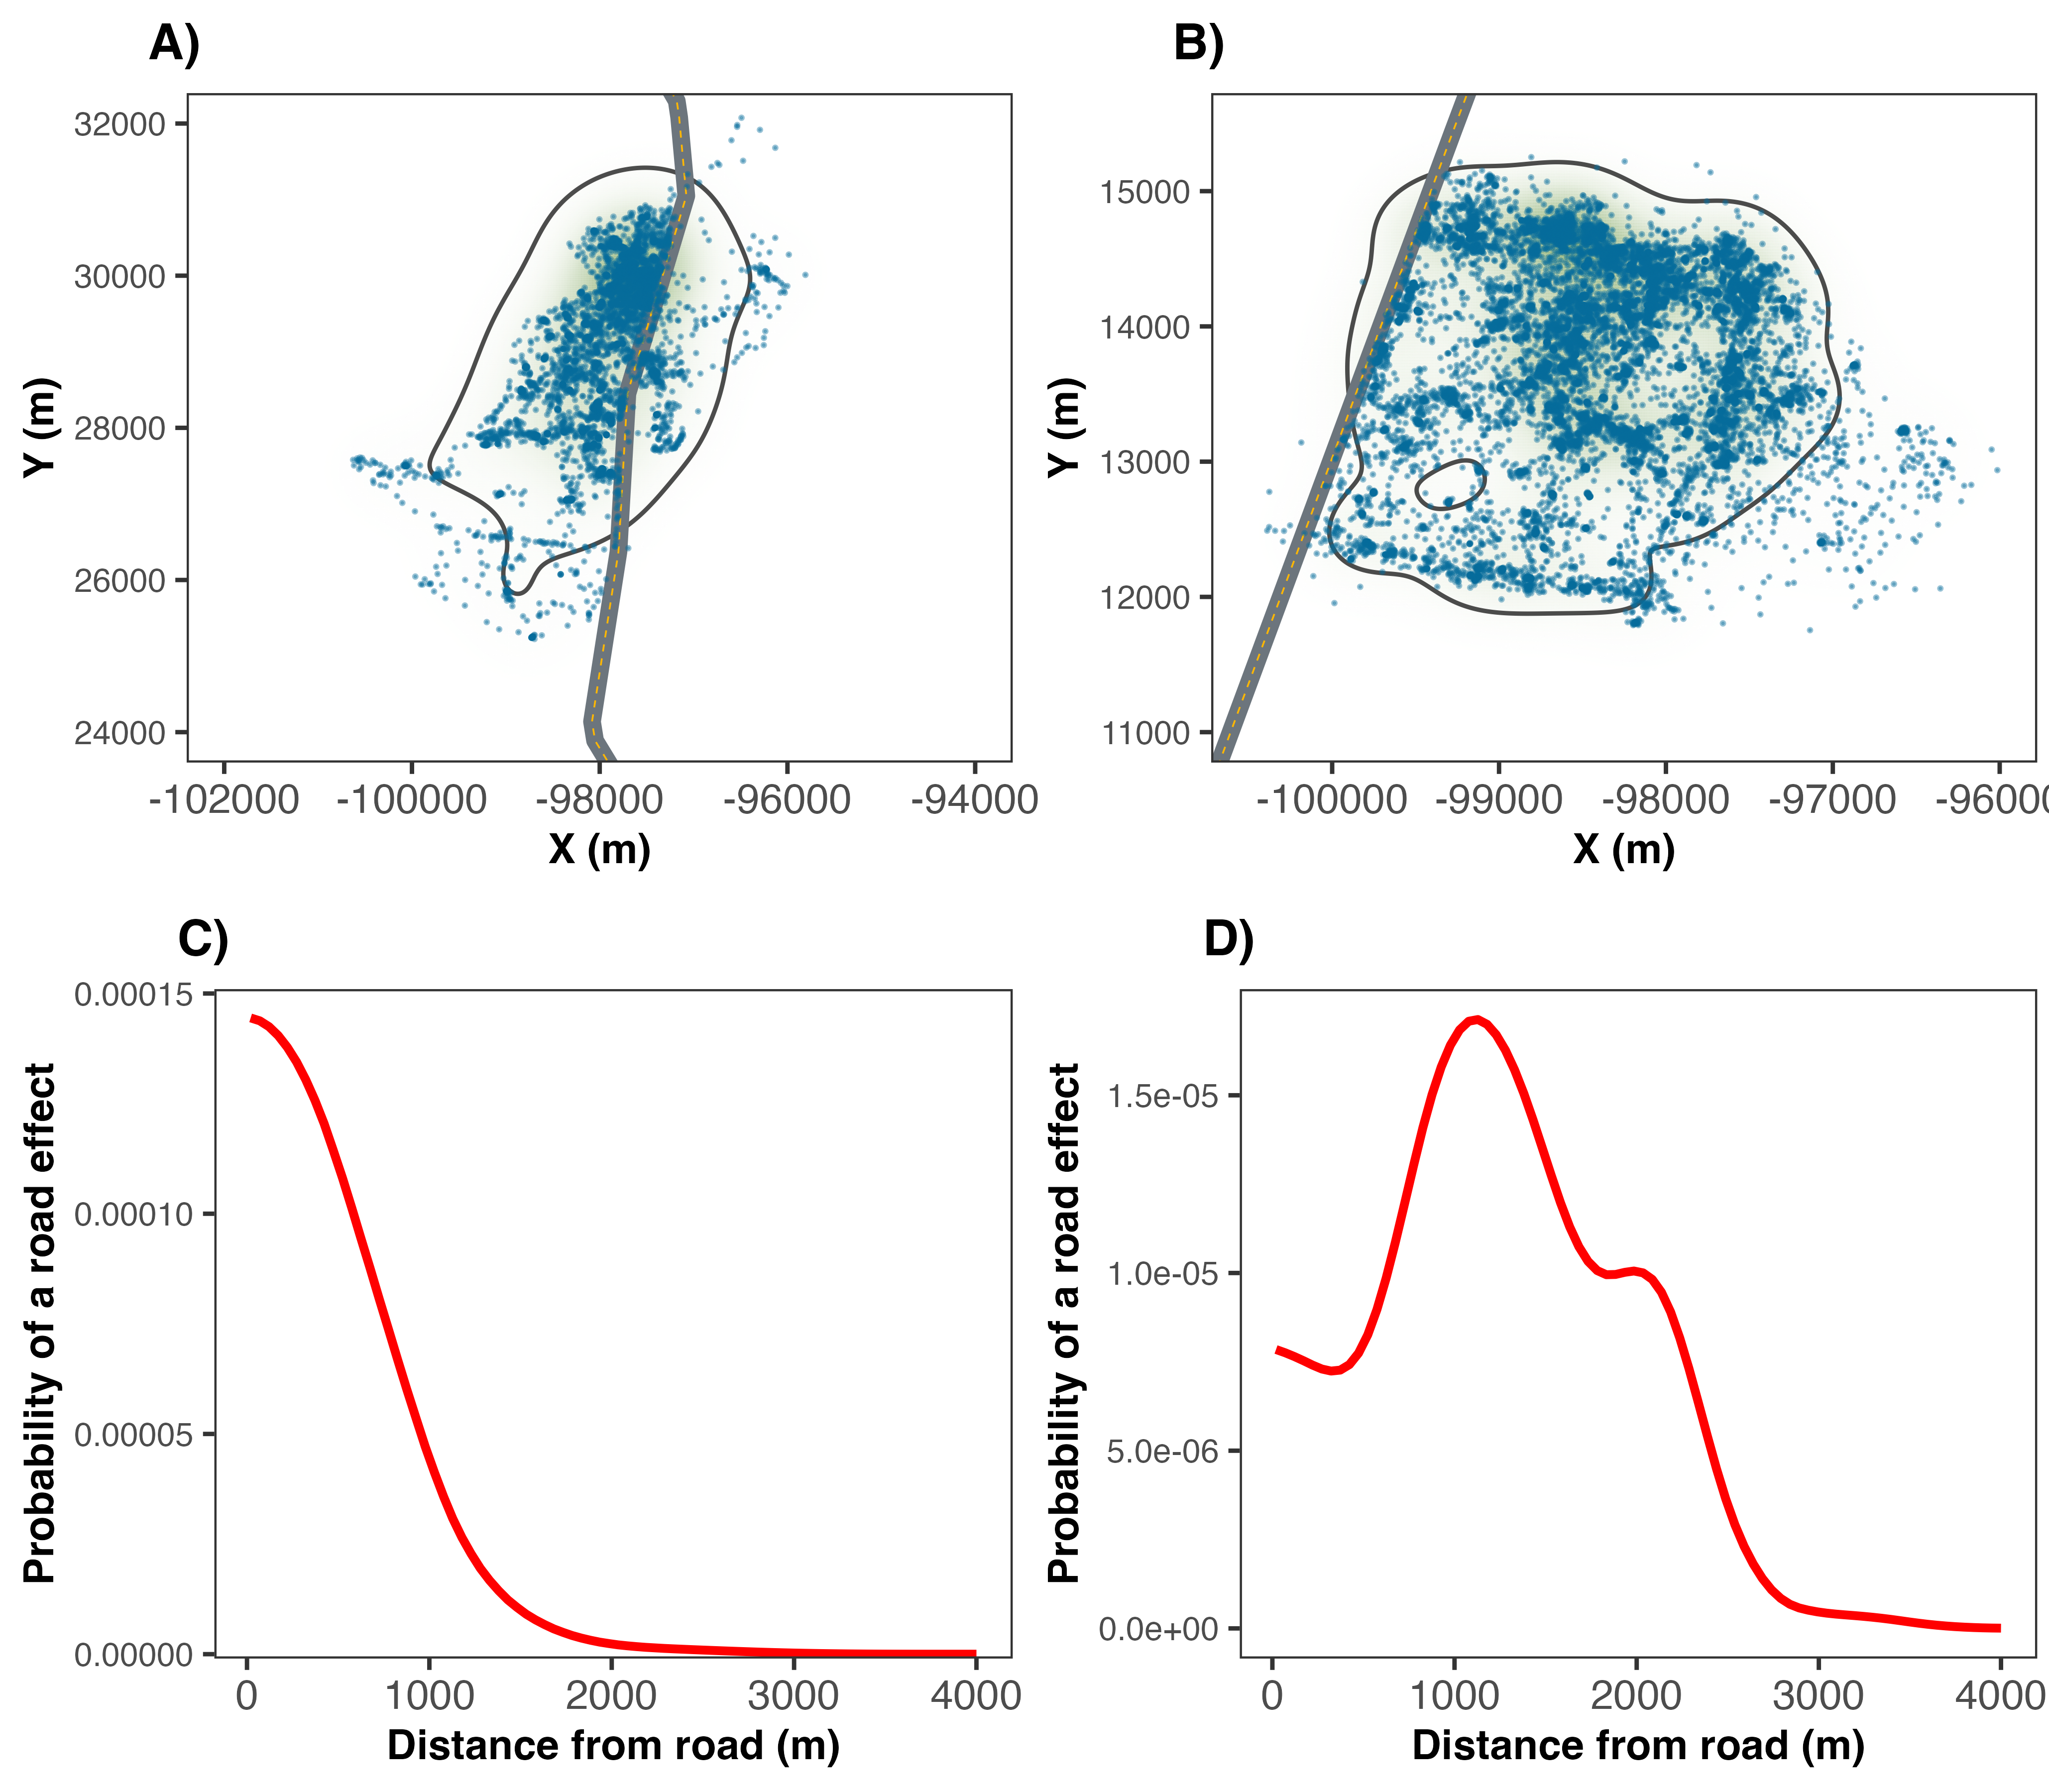
\includegraphics[scale= 0.9]{Anteater_RE}
\caption{The relationship between space use and the road effect zone for two giant anteaters in the Brazilian Cerrado. Note how in panel A), the animal lives right along the roadside, so the ecological effects of a road mortality are greatest near the road, as shown in panel C). In Panel B), the animal's home range was further from the road and while the overall road effect was weaker, it peaked between 1-2km from the road.}
\end{figure}

\begin{figure}[h!]
%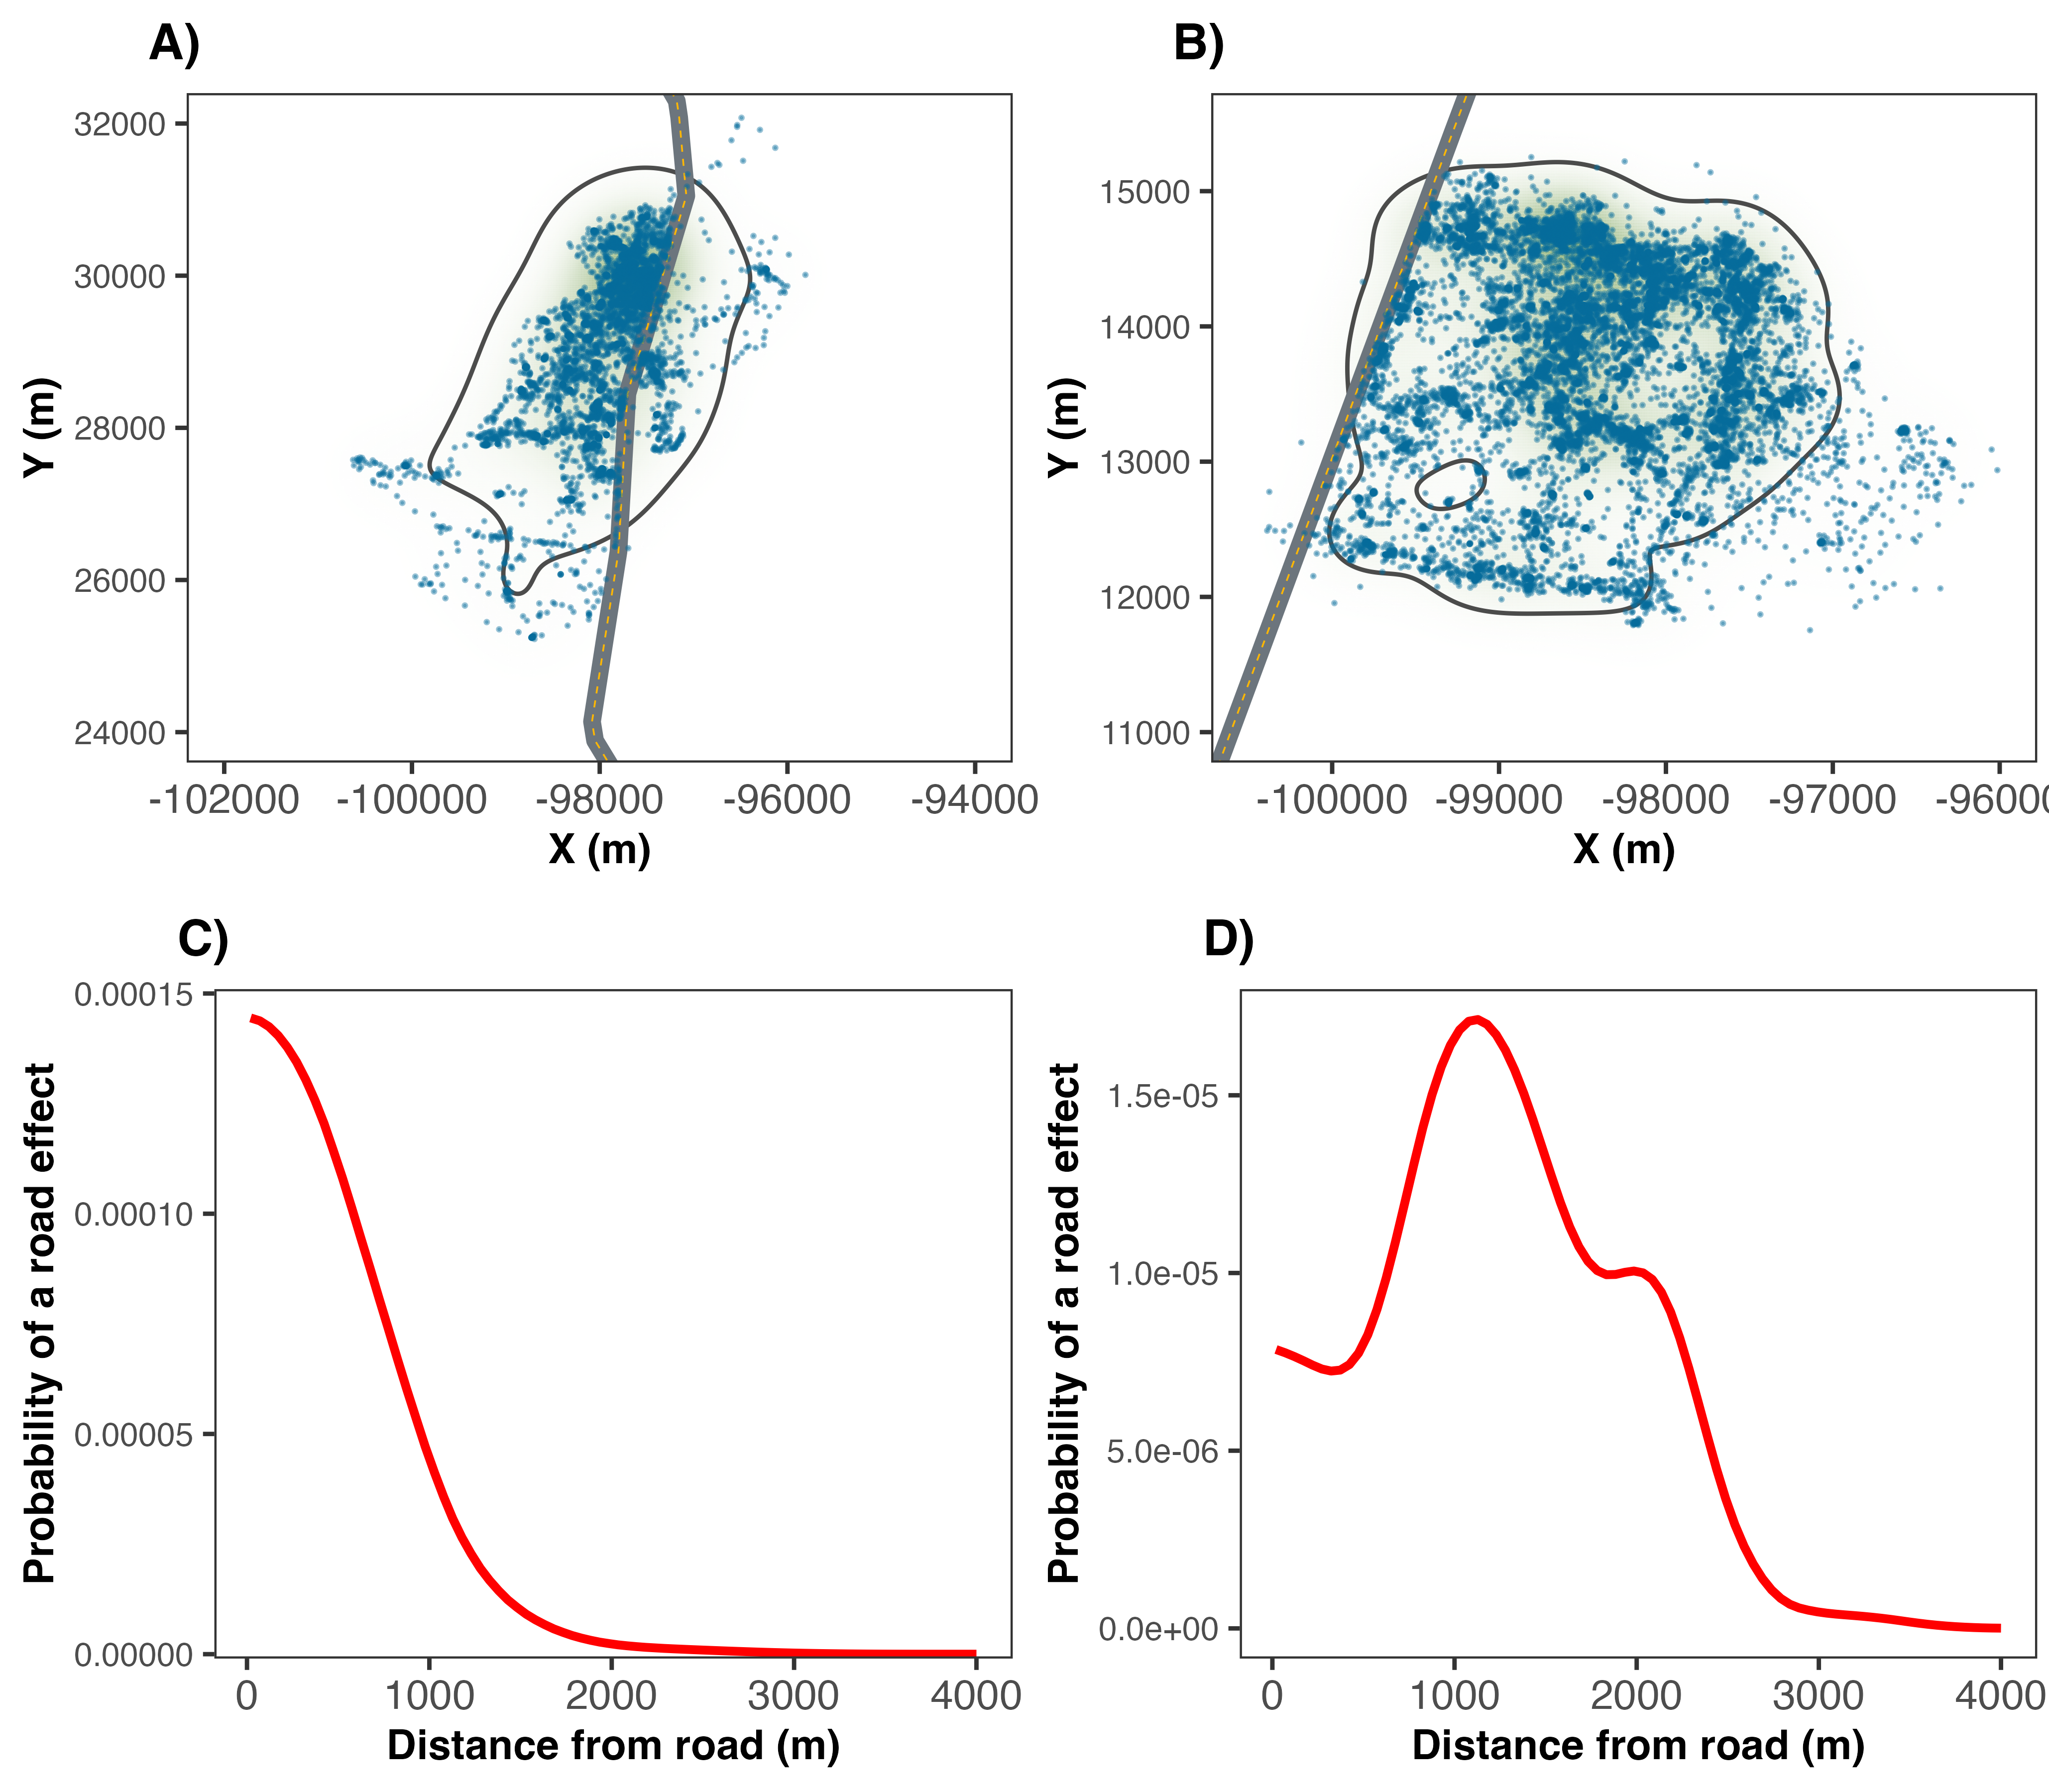
\includegraphics[scale= 0.9]{Anteater_RE}
\caption{The relationship between space use and the road effect zone for two giant anteaters in the Brazilian Cerrado. Note how in panel A), the animal lives right along the roadside, so the ecological effects of a road mortality are greatest near the road, as shown in panel C). In Panel B), the animal's home range was further from the road and while the overall road effect was weaker, it peaked between 1-2km from the road.}
\end{figure}


\end{document}
